%%%
% Approach for Interactive Diagram-Specific Layout of Graph-based Software Diagrams
%%%

\chapter{Ansatz für das interaktive und diagrammspezifische Layout von graph-basierten Softwarediagrammen}
\label{chapter:interactive-approach}

In diesem Kapitel wird ein Ansatz für das interaktive und diagrammspezifische Layout von Diagrammen präsentiert. Zunächst werden im Abschnitt \ref{sec:requirements-analysis} die Kriterien aufgestellt. Die grundlegende Funktionsweise wird im Abschnitt \ref{sec:interactive-approach-functionality} erklärt. Eine detaillierte Beschreibung der Layout-Patterns und deren Rolle in dem präsentierten Ansatz folgt im Abschnitt \ref{sec:layout-patterns}.
% TODO: Aufbau des Kapitels ergänzen!

\section{Kriterien}
\label{sec:requirements-analysis}

Im Folgenden werden Kriterien für den präsentierten Ansatz aufgestellt. Die Wahl der Kriterien stützt sich in erster Linie auf die Prinzipien für die agile Modellierung aus \cite{Ambler02Agile}. Weiterhin orientieren sich die Kriterien an den im Kapitel \ref{chapter:existing-approaches} vorgestellten Ansätzen, deren positiven Eigenschaften in die Auswahl einfließen.   Schließlich haben auch die ästhetischen Prinzipien (siehe Abschnitt \ref{sec:aesthetics-criteria}) sowie die Rahmenbedingungen dieser Arbeit (siehe Abschnitt \ref{sec:conditions}) einen Einfluss auf die gewählten Kriterien.

\begin{enumerate}[label={K.\arabic*}]
    \item \label{req:gui} \textbf{GUI} Wie bereits im Abschnitt \ref{sec:conditions} erwähnt, beschäftigt sich diese Arbeit ausschließlich mit Mechanismen für das Layout von Diagrammen, die in Tools für klassische grafische Benutzeroberflächen eingesetzt werden. Daher soll der Ansatz für klassische grafische Benutzeroberflächen ausgelegt sein und von üblichen GUI-basierten Bedientechniken wie z.B. \enquote{Drag and Drop} Gebrauch machen.
    \item \label{req:interactivity} \textbf{Interaktivität} Die Manipulation mit dem Diagramm soll interaktiv erfolgen. Der Nutzer soll in der Lage sein, mit dem Diagramm unmittelbar interagieren zu können und die Layout-Anpassungen sollen eine direkte Auswirkung auf das manipulierte Diagramm haben. Demzufolge soll die Eingabe mit der Ausgabe fest gekoppelt sein\footnote{Dies bezieht sich auf das GUI-Tool, das den Ansatz implementiert. Aus der Sicht der Mensch-Computer-Interaktion ist die Nutzung der Maus als Eingabegerät von der Ausgabe am Monitor stets entkoppelt.}.
    \item \label{req:editing-support} \textbf{Förderung des Prozesses der Diagramm-Erstellung} Der Nutzer soll den Inhalt des Diagramms bearbeiten und inkrementell modifizieren können \cite{GladischSchumann14Semi-Automatic}. Dabei soll das Layout nach jeder Änderung des Inhalts angepasst werden. Weiterhin soll es möglich sein, das Layout des Diagramms bis zu einem bestimmten Grad nach den Präferenzen des Nutzers beeinflussen zu können.
    \item \textbf{Erhaltung des mentalen Modells} Die Layout-Änderungen im Diagramm sollen möglichst intuitiv erfolgen, insbesondere soll das mentale Modell erhalten werden (siehe Abschnitt \ref{subsec:mental-map}).
    
    \item \label{req:focus-on-the-content} \textbf{Förderung der Konzentration auf den Inhalt} Der Inhalt eines Diagramms soll eine wichtigere Rolle als seine Repräsentation haben \cite[S.38ff]{Ambler02Agile}. Diese Tatsache soll in dem Ansatz berücksichtigt werden, indem der Aufwand für das Erzeugen des Layouts verringert wird. Außerdem sollen die Aktionen zur Anpassung der visuellen Eigenschaften möglichst eingeschränkt sein.
    \item \label{req:aesthetics-criteria} \textbf{Berücksichtigung der ästhetischen Prinzipien} Die Layout-Berechnung soll unter Berücksichtigung der im Abschnitt \ref{sec:aesthetics-criteria} beschriebenen ästhetischen Prinzipien für graph-basierte Softwarediagramme erfolgen.
    \item \textbf{Berücksichtigung der Syntax und Semantik} Die Syntax- und Semantikregeln der einzelnen Diagrammtypen sollen berücksichtigt werden und es sollte nicht möglich sein, diese Regeln zu verletzen. 
    % TODO: Meta-Modell erwähnen, Verletzen der Regeln
       
%    \item \label{req:user-friendly} \textbf{Benutzerfreundlichkeit} Der Ansatz soll möglichst benutzerfreundlich sein. Insbesondere ist wichtig, dass die Einschränkungen bzgl. des Layouts nicht zur Frustration des Nutzers führen.
\end{enumerate}
    
\section{Funktionsweise}
\label{sec:interactive-approach-functionality}

\subsection{Bearbeitungsaktionen}

Alle interaktiven Ansätze für das Layout von Diagrammen aus dem Kapitel \ref{chapter:existing-approaches} bis auf das \enquote{Smart Layout} in MindNode (siehe Abschnitt \ref{subsubsec:smart-layout-in-mindnode}) unterstützen eine \textbf{freie Positionierung} der Objekte im Diagramm. Diese Art der Bedienung wird im manuellen Layout zusätzlich um temporäre Hilfefunktionen (siehe Abschnitt \ref{sec:manual-layout}) und in Struktur-basierten benutzergesteuerten Ansätzen um Möglichkeit der Erzeugung von Strukturregeln (siehe Abschnitt \ref{subsec:structure-based-user-controlled-approaches}) erweitert. Durch diese Erweiterungen wird die freie Positionierung eingeschränkt, dass in der Regel zu einem besseren Layout des Diagramms führt. Dahingegen ist die freie Positionierung in \enquote{Smart Layout} in MindNode und dem in dieser Arbeit präsentierten Ansatz nicht gestattet. Somit bewirkt die Verschiebung eines Objekts im Diagramm keine direkte Anpassung seiner Position, sondern wird als eine Äußerung der gewünschten Position interpretiert.

Die Kriterien \ref{req:interactivity} und \ref{req:editing-support} erfordern eine interaktive Bearbeitung des Diagramms. Dies wird in dem Ansatz durch die Unterstützung von \textbf{Bearbeitungsaktionen} gewährleistet, die durch den Nutzer ausgeführt werden können. Diese lassen sich in zwei Gruppen unterteilen. Zu einem sind das Aktionen, die den Inhalt des Diagramms modifizieren (z.B. Hinzufügen oder Löschen eines Objekts) und zu anderem sind das Aktionen, die das Layout des Diagramms modifizieren, ohne den Inhalt zu verändern (z.B. Verschiebung eines Objekts).

Die interaktiven Ansätze werden in Editoren eingesetzt, die in der Regel über einen \enquote{Canvas} verfügen. Der Canvas ist ein rechteckiger Bereich des Editor-Fensters, in dem das Diagramm dargestellt wird und in dem die Interaktion mit dem Diagramm durch die Ausführung von Bearbeitungsaktionen stattfindet. Obwohl in den meisten Editoren die Reihenfolge der Objekte im Canvas festgelegt werden kann und der Canvas somit mehrschichtig erscheint, handelt es sich aus der Sicht der Interaktion lediglich um eine Schicht.

%Alle im Kapitel \ref{chapter:existing-approaches} vorgestellten interaktiven Ansätzen sind für eine
%\footnote{Eine Ausnahme bildet das Hinzufügen von Objekten in einigen Programmen (z.B. Keynote und Visual Paradigm).}
%\footnote{Durch die Funktionen... und durch das Erstellen von expliziten Schichten \cite{08OmniGraffle}..}, 

Für die Umsetzung der Bearbeitungsaktionen unter Berücksichtigung der Einschränkung der Positionierung der Objekte ist der Einsatz eines neuen Mechanismus erforderlich, der die Grundlage des präsentierten Ansatzes bildet. Dieser Mechanismus macht sich die Technik \enquote{Drag and Drop} zu Nutze und führt eine zweite Schicht der Interaktion vor der Schicht des Canvas ein. Somit wird bei dem \enquote{Drag} eines Objekts aus dem Canvas seine Repräsentation zu einem Platzhalter (dargestellt mit gestrichelten Linien) umgewandelt und eine weitere Repräsentation in der neu eingeführten Schicht erzeugt. Dieser Sachverhalt wird in Abbildung \ref{fig:two-layers-mechanism} dargestellt.

\begin{figure}[hbt]
    \newcommand{\subfigurewidth}{0.35\textwidth}
    \newcommand{\graphicsscale}{1.2}
    \centering
    \begin{subfigure}{\subfigurewidth}
        \centering
        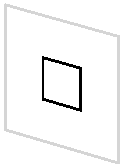
\includegraphics[scale=\graphicsscale]{resources/two-layers-mechanism-a}
        \caption{Ein Objekt im Canvas}
    \end{subfigure}
    \begin{subfigure}{\subfigurewidth}
        \centering
        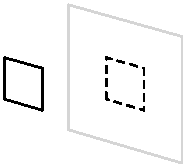
\includegraphics[scale=\graphicsscale]{resources/two-layers-mechanism-b}
        \caption{}
    \end{subfigure}
    \caption{Mechanismus der Einführung einer zweiten Schicht für \enquote{Drag and Drop}}
    \label{fig:two-layers-mechanism}
\end{figure}




%und wird insbesondere bei der Verschiebungsoperation eingesetzt (siehe Abschnitt X)


\subsection{Layout-Engine}

% operiert auf dem CSM, verändert die Layout-Eigenschaften
% graph-basierte Diagramme: Knoten und Kanten
% Layout-Übergänge

\subsection{Auswertung der Verschiebungsaktion}

% Auswertung der Verschiebungsaktion
% ursprünglicher Ansatz





% Für jede Bearbeitungsaktion wird ein Layout-Ereignis erzeugt, das neben der Information über die manipulierten Objekte auch Parameter der Interaktion besitzt.


% Auswertung der Layout-Ereignissen durch die Layout-Engine und eventuelle Anpassung des Layouts








% Einschränkung der Aktionen, die der Nutzer ausführen kann

% Abnehmen der Layout-Arbeit durch Einschränkung der Flexibilität

% Herausforderung bei der Kombination von mehreren Kriterien (z.B. interaktive Bedienung aber gleichzeitig eine Einschränkung der Möglichkeiten)
% optimales Verhältnis zwischen flexiblen Modifizierungen der Layout-Eigenschaften und ...





%die Vorteile der freien Positionierung der Elemente im Diagramm und der automatischen Layout-Algorithmen miteinander kombiniert. Unter Berücksichtigung des Diagrammtyps werden durch einen Algorithmus mögliche Layouts berechnet. Der Nutzer wird in der Lage sein, durch Interaktion mit dem Diagramm das passende Layout auszuwählen und neue Elemente zu dem Diagramm hinzuzufügen.

%%%%%%%%%

% Spezialisierung, Einschränkung, Interaktivität

%Durch die Spezialisierung auf konkrete Diagramm-Typen und den Einsatz von verschiedenen Vereinfachungsmaßnahmen wie etwa Einschränkung der unterstützten Notation \cite[S.56ff]{Ambler02Agile} lassen sich Algorithmen für das Layout von Softwarediagrammen entwerfen, die zwar nicht so flexibel wie z.B. \cite{Maier12A-Pattern-based} oder \cite{Eichelberger05Aesthetics} sind, aber dafür...




% Einschränkung der Möglichkeiten, Berücksichtigung der Syntax und Semantik der Diagramme


% unmittelbares vs. verzögertes Feedback [Wybrow S.69]
% kombiniert Vorteile der freien Positionierung der Elemente im Diagramm und der automatischen Layout-Algorithmen miteinander

% Drag&Drop-Technik (neue Elemente aus einer Palette bzw. Änderung des Layout im Diagramm)

% Animation
% Mentales Modell [Maier, Wybrow?]




%\section{Definitionen}

% Layout
% Layout-Übergang
% Layout-Pattern
% Layout-Ereignis


% Layout-Engine
% =============
% Eingabe für den Algorithmus: Layout-Ereignis, Inhalt des Diagramms, instanziierte Patterns, der Layout-Zustand (mögliche Layout-Übergänge vom aktuellen Zustand abhängig, nicht alle erreichbar)
% berechnete Layouts = Positionen für Knoten, Routen für Kanten (nicht implementiert), Animationen/Übergangsparameter für die Transitionen (nicht implementiert)
% initialer Zustand

% Erreichbare Layouts werden berechnet und mit Hilfe der Layout-Ereignisse wird geprüft, ob ein Layout-Übergang stattfinden soll (z.B. nur die benachbarten Bereiche im horizontalen Layout-Algorithmus)
% nach einem Layout-Übergang wird die Berechnung wiederholt

% Layout-Engine soll für spezielle Diagrammtypen unterschiedliches Verhalten aufweisen
% Jeder Diagrammtyp (z.B. Klassendiagramm, Zustandsdiagramm, Flowchart usw.) hat aufgrund der Semantik- und Strukturregeln spezielle Anforderungen an das ästhetische Layout
% automatische Instanziierung von Patterns nach Layout-Ereignissen
% Neu-Berechnung nach jedem Layout-Übergang -> Performance?
% Stabilität -> Ausführen eines Layout-Übergangs nach einer deutlichen Aktion des Nutzers
% Erreichbarkeit des Ausgangslayouts

% In Rahmen der Konzeption und Entwicklung wurde zunächst ein Algorithmus entworfen, der für die Manipulation eines Knotens alle möglichen Layouts und die entsprechenden Diagramm-Bereiche für das gesamte Diagramm explizit berechnet hat. Durch eine Bewegung des Mauszeigers in einen anderen Bereich wurde jeweils ein Layout-Übergang ausgelöst. Die Berechnung wurde jedoch nicht nach jedem Layout-Übergang wiederholt und die Abbildung war oft nach dem ersten Layout-Übergang ungültig. Später wurde festgelegt, dass dieser Algorithmus nicht hinreichend ist.

\section{Layout-Patterns}
\label{sec:layout-patterns}

% Abgrenzung des Begriffs zu dem von [Maier]
% implizite vs. explizite Layout-Patterns (siehe Mappe)
% Patterns-Variierung (z.B. Reihenfolge der Knoten kann von Nutzer festgelegt werden, das endgültige Layout wird durch die Geometrie bestimmt)
% instanziiert in der Layout-Engine, referenzieren den Diagramm-Inhalt
% Wiederverwendung möglich (mehrere Instanzen in der Layout-Engine bzw. Komposition von Patterns wie T-Shape-Pattern)
% Nur während Drag&Drop sichtbar -> Möglichkeit der Interaktivität der Patterns
% interne Berechnung des relativen Layouts für enthaltene Diagramm-Objekte (Knoten)

% konkrete Pattens:
% - detaillierte Beschreibung der expliziten Layout-Patterns mit Bezug auf Arbeiten
% - Erläutern der geometrischen Parametern mit Bildern
% - Bild mit Instanzen von Patterns in einem Beispiel-Diagramm (kann ein Screenshot sein)
% - IDLPattern, IDLAlignmentPattern, IDLTShapePattern -> Klassendiagramm

% Instanziierung durch den Nutzer wie in [Maier] ist denkbar

\subsection{Implizite Layout-Patterns}

\subsubsection{Größe der Knoten}
\subsubsection{Zentrierung des Inhalts}
\subsubsection{Gleiche Abstände}
\subsubsection{Verhinderung der Knoten-Überlappung}

\subsection{Explizite Layout-Patterns}

% TODO: Verweis auf die implementierten Patterns im Prototypen (Kapitel 5) hinzufügen
% Variationen der expliziten Layout-Patterns

\subsubsection{Ausrichtung}

% siehe manuelles Layout bzw. Pattern-basierter Ansatz (Kapitel 3)
% gleichmäßige Verteilung (Abstände gleich groß)
% Variationen: Reihenfolge der Knoten

\subsubsection{T-Shape}

% Variationen: Reihenfolge der Knoten im Ausrichtungs-Pattern
% interne Wiederverwendung eines Ausrichtung-Patterns





\section{Abgrenzung zu bestehenden Ansätzen}

% Was ist neu an dem Ansatz?
% Vergleich zu bestehenden Ansätzen im Kapitel 3
% Worin unterscheidet sich mein Ansatz zu dem von Sonja Maier?
% - Drag&Drop mit Visualisierung der Aktion
% - Kein Freihand-Editieren, sondern implizite Bereiche und Layout-Übergänge
% - Patterns unterstützen Variierung
% - Starke Vereinfachung der Möglichkeiten (Anpassung der Patterns aus [Maier])
